\chapter{Basic linear algebra}

Basic linear algebra is super fundamental to what this package does,
so we will give an overview of the prerequisites here. My hope is that
this chapter will be short and accessible, with just enough core concepts 
to do pretty much whatever we want down the road. Linear algebra can become 
quite memory intensive if we look at a typical university curriculum. I have 
deliberately chosen to write this chapter in a more immediately accessible
way, with just some core concepts.

\section{Linear operations on geometric-coordinate vectors}

In basic linear algebra, vectors are typically introduced in a more 
conceptually intuitive way. Specifically, they are commonly represented 
as directed line segments. This is a geometric-coordinate vector.
Vectors can be much more abstract than this,
but that is not basic linear algebra. 

Then the student is introduced to 
operations on these vectors. An operation can take one or more operand,
and in the case of linear operations, these operands are vectors. However,
there are operations later on down the road which accept operands of different 
types, so this isn't a rule. 

The linear operations achieve intuitive geometric effects, such as measuring 
distances, angles, or even producing new vectors with special properties 
relative to the operands; e.g., orthogonality.

\subsection{Geometric-coordinate vectors in 3D}

A geometric-coordinate vector in 3D is any 
element of the collection of 3-arrays of 
numbers and unique coordinates in 3-space, 
which are bijectively related.
This is a bunch of jargon which says that 
every sequence of 3 numbers 
corresponds to exactly one coordinate in 
3-space. This is not a rigorous explanation,
but I hope that it lands instead on a more 
intuitive basis. See Figure~\ref{fig:la1}.

\begin{figure}
    \centering 
    \begin{tikzpicture}[scale=0.7]
        \ltdtsetobject[
            name=view,
            object={
                return Matrix.zyzrotation(
                    Vector:new{pi/6,pi/3,pi/2}
                )
            }
        ]
        \ltdtappendlight[v={return Vector:new{1,1,1,1}}]

        % axes
        \ltdtappendcurve[
            uparams={return Vector:new{0,1,2}},
            v={return Vector:new{u,0,0,1}:hscale(5)},
            arrow tip={return "fill=ltdtbrightness"},
            % arrow tail={return "fill=ltdtbrightness"},
            draw options={return "draw,line cap=round"},
            transformation={return view}
        ]
        \ltdtappendcurve[
            uparams={return Vector:new{0,1,2}},
            v={return Vector:new{0,u,0,1}:hscale(5)},
            arrow tip={return "fill=ltdtbrightness"},
            draw options={return "draw,line cap=round"},
            transformation={return view}
        ]
        \ltdtappendcurve[
            uparams={return Vector:new{0,1,2}},
            v={return Vector:new{0,0,u,1}:hscale(5)},
            arrow tip={return "fill=ltdtbrightness"},
            draw options={return "draw,line cap=round"},
            transformation={return view}
        ]
        \ltdtappendlabel[
            text={\(x\)},
            v={return Vector:new{6,0,0,1}},
            transformation={return view}
        ]
        \ltdtappendlabel[
            text={\(y\)},
            v={return Vector:new{0,6,0,1}},
            transformation={return view}
        ]
        \ltdtappendlabel[
            text={\(z\)},
            v={return Vector:new{0,0,6,1}},
            transformation={return view}
        ]

        \ltdtappendcurve[
            uparams={return Vector:new{0,1,2}},
            v={return Vector:new{u/2,u/3,u/4,1}:hscale(5)},
            arrow tip={return "fill=ltdtbrightness!50!red"},
            draw options={return "draw=red,line cap=round"},
            transformation={return view}
        ]
        \ltdtappendcurve[
            uparams={return Vector:new{0,1,2}},
            v={return Vector:new{1/2,1/3,u/4,1}:hscale(5)},
            draw options={return "draw=red,line cap=round,dashed"},
            transformation={return view}
        ]
        \ltdtappendcurve[
            uparams={return Vector:new{0,1,2}},
            v={return Vector:new{u/2,1/3,0/4,1}:hscale(5)},
            draw options={return "draw=red,line cap=round,dashed"},
            transformation={return view}
        ]
        \ltdtappendcurve[
            uparams={return Vector:new{0,1,2}},
            v={return Vector:new{1/2,u/3,0/4,1}:hscale(5)},
            draw options={return "draw=red,line cap=round,dashed"},
            transformation={return view}
        ]
        \ltdtdisplaysimplices
    \end{tikzpicture}
    \caption{A geometric-coordinate vector in 3D}
    \label{fig:la1}
\end{figure}

\subsection{Addition and scalar multiplication}

We can add and scale geometric-coordinate vectors.
When we add them coordinate-wise, we add the components.
This corresponds to geometric-wise addition where we 
connect the tail of the second vector to the tip of 
thefirst vector and produce the vector from the first's 
tail to the second's tip. For example,
\[
    \begin{bmatrix}
        1 \\ 2 \\ 3
    \end{bmatrix}
    +
    \begin{bmatrix}
        2 \\ 2 \\ 1
    \end{bmatrix}
    =
    \begin{bmatrix}
        3 \\ 4 \\ 4
    \end{bmatrix}.
\] See Figure~\ref{fig:la2}.
Similarly, we scale vectors coordinate-wise by scaling each element uniformly.
Geometrically, this produces a vector which points in the same direction, and 
has its length uniformly scaled.

\begin{figure}
    \centering 
    \begin{tikzpicture}[scale=0.7]
        \ltdtsetobject[
            name=view,
            object={
                return Matrix.zyzrotation(
                    Vector:new{7*pi/6,pi/3,pi/2}
                )
            }
        ]
        \ltdtappendlight[v={return Vector:new{1,1,1,1}}]
        \ltdtappendcurve[
            uparams={return Vector:new{0,1,2}},
            v={return Vector:new{u/2,u/3,u/4,1}:hscale(5)},
            arrow tip={return "fill=ltdtbrightness!50!red"},
            draw options={return "draw=red,line cap=round"},
            transformation={return view}
        ]
        \ltdtappendcurve[
            uparams={return Vector:new{0,1,2}},
            v={
                return Vector:new{1/2,1/3,1/4,1}
                :hadd(Vector:new{u,-u/4,-u/2,1})
                :hscale(5)
            },
            arrow tip={return "fill=ltdtbrightness!50!red"},
            draw options={return "draw=red,line cap=round"},
            transformation={return view}
        ]
        \ltdtappendcurve[
            uparams={return Vector:new{0,1,2}},
            v={
                return Vector:new{1/2,1/3,1/4,1}
                :hadd(Vector:new{1,-1/4,-1/2,1})
                :hscale(5*u)
            },
            arrow tip={return "fill=ltdtbrightness!50!green"},
            draw options={return "draw=green,line cap=round"},
            transformation={return view}
        ]
        \ltdtdisplaysimplices
    \end{tikzpicture}
    \caption{Geometric-coordinate vector addition in 3D}
    \label{fig:la2}
\end{figure}

\subsection{Dot and cross products}

The dot product is useful for measuring angles and directional distances.
It is written as follows;
\[
    \begin{bmatrix}
        1 \\ 2 \\ 3
    \end{bmatrix}
    \cdot 
    \begin{bmatrix}
        2 \\ 2 \\ 1
    \end{bmatrix}
    =
    \begin{bmatrix}
        1\cdot2 \\ 2\cdot2 \\ 3\cdot1
    \end{bmatrix}
    =
    \Biggl\lVert
    \begin{bmatrix}
        1 \\ 2 \\ 3
    \end{bmatrix}
    \Biggr\rVert
    \Biggl\lVert
    \begin{bmatrix}
        2 \\ 2 \\ 1
    \end{bmatrix}
    \Biggr\rVert
    \cos(\mbox{ least angle }).
\]

The cross product is a means of achieving orthogonality.
It has a formula, but the formula is unmemorizable.
It could be derived by a determinant of a vector valued matrix,
but that would be too expensive in terms of speed. So, we will be 
geometric here, instead of numeric. In Figure~\ref{fig:la3},
the area of the red region is the dot product, and the cross product is 
the blue vector and its length is the area of the blue region.

\begin{figure}
    \centering
    \begin{tikzpicture}[scale=0.5]
        \pgfmathsetmacro\i{15*2*pi/40}
        \ltdtsetobject[
            name=view,
            object={
                return Matrix.zyzrotation(
                    Vector:new{7*pi/6,pi/3,pi/2}
                )
            }
        ]
        \ltdtappendlight[v={return Vector:new{1,1,1,1}}]
        \ltdtappendcurve[ % VECTOR U
            uparams={return Vector:new{0,1,2}},
            v={return Vector:new{u*cos(0),u*sin(0),0,1}:hscale(2)},
            arrow tip={return "fill=ltdtbrightness"},
            draw options={return "draw,line cap=round"},
            transformation={return view}
        ]
        \ltdtappendlabel[
            text={\(\vec{u}\)},
            transformation={return view},
            v={return Vector:new{cos(0),sin(0),0,1}:hscale(2.25)}
        ]
        \ltdtsetobject[
            name={vecV},
            object={
                return Vector:new{cos(\i),sin(\i),0,1}
                :hscale(1.3+sin(\i)/5)
            }
        ]
        \ltdtappendcurve[ % VECTOR V
            uparams={return Vector:new{0,1,2}},
            v={return Vector:new{u,u,0,1}:hinnervec(vecV):hscale(3)},
            arrow tip={return "fill=ltdtbrightness"},
            draw options={return "draw,line cap=round"},
            transformation={return view}
        ]
        \ltdtappendlabel[
            text={\(\vec{v}\)},
            transformation={return view},
            v={return vecV:hscale(3.25)}
        ]
        \ltdtappendcurve[ % VECTOR UxV
            uparams={return Vector:new{0,1,2}},
            v={
                return Vector:new{u*cos(0),u*sin(0),0,1}:hscale(2)
                :hcross(Vector:new{u,u,0,1}:hinnervec(vecV):hscale(3))
            },
            arrow tip={return "fill=ltdtbrightness!50!cyan"},
            draw options={return "draw=cyan,line cap=round"},
            transformation={return view}
        ]
        \ltdtappendlabel[
            text={\(\vec{u}\times\vec{v}\)},
            transformation={return view},
            v={
                return Vector:new{cos(0),sin(0),0,1}:hscale(2)
                :hcross(vecV:hscale(3)):hscale(1.15)
            }
        ]
        \ltdtappendsurface[ % CROSS PRODUCT
            uparams={return Vector:new{0,1,2}},
            vparams={return Vector:new{0,1,2}},
            v={
                return Vector:new{u*cos(0),u*sin(0),0,1}:hscale(2)
                :hadd(Vector:new{v,v,0,1}:hinnervec(vecV):hscale(3))
            },
            transformation={return view},
            fill options={
                return [[
                    fill=ltdtbrightness!50!cyan,
                    fill opacity=0.3
                ]]
            }
        ]
        \ltdtappendsurface[
            uparams={return Vector:new{0,1,2}},
            vparams={return Vector:new{0,1,2}},
            v={
                return Vector:new{cos(-pi/2),sin(-pi/2),0,1}:hscale(vecV:hscale(3):norm()*u)
                :hadd(Vector:new{cos(\i),sin(\i),0,1}:hscale(2*v))
            },
            transformation={return view},
            fill options={
                return [[
                    fill=ltdtbrightness!50!red,
                    fill opacity=0.3
                ]]
            }
        ]
        \ltdtappendcurve[
            uparams={return Vector:new{0,1,40}},
            v={return Vector.sphere(Vector:new{u*tau,pi/2,2})},
            transformation={return view},
            draw options={return "draw=black,line cap=round"}
        ]
        \ltdtdisplaysimplices
    \end{tikzpicture}
    \caption{The dot product (red) and cross product (blue)}
    \label{fig:la3}
\end{figure}

\section{Linear combinations of geometric vectors}

Arrows (an informal, yet intuitive terminology) are very useful for 
\textbf{navigating subspaces}. A subspace can be a point, line, or plane 
which passes through the origin. In the chapter on affine algebra, we 
will extrapolate this concept to affine subspaces which do not necessarily 
coincide the origin. The steering wheel we use is called a linear combination 
of a linear basis. The linear basis is the set of directions we can travel,
and the combination is the sum of them, each scaled by various lengths.
Recall that summing scaled vectors lets us traverse space by their length and 
direction.

\section{Navigating subspaces using bases}

A 3D linear subspace basis is a matrix of zero, one, or two 3-tuples.
These vectors absolutely cannot be redundant. There must be a bijection 
between every linear combination and every point in the subspace.
That's a bit fancy language, but it means they must be one for one.

\section{Intersections of subspaces}

We use Gauss Jordan elimination to identify intersections of subspaces.
You do not need to know how to compute column reduction fot this software.
See Figure~\ref{fig:la4}. For example, if we have two plane equations,
we can use column reduction---row reduction is more common, but harder to type---
to determine the subspace through which they intersect. Subspaces always 
intersect in lower dimensional subspaces.

\begin{figure}
    \centering
    \begin{tikzpicture}
        \ltdtsetobject[
            name=view,
            object={
                return Matrix.zyzrotation(
                    Vector:new{7*pi/6,pi/3,pi/2}
                )
            }
        ]
        \ltdtsetobject[
            name=cam,
            object={return view:inverse()}
        ]
        \ltdtappendlight[
            v={return Vector:new{1,1,1,1}}
        ]
        \ltdtappendsolid[
            uparams={return Vector:new{-2,2,2}},
            vparams={return Vector:new{-2,2,2}},
            wparams={return Vector:new{-2,2,2}},
            v={return Vector:new{u,v,w,1}},
            transformation={return view},
            fill options={
                return [[
                    draw=black,
                    fill=ltdtbrightness!20!gray,
                    fill opacity=0.08
                ]]
            }
        ]
        \foreach \i in {1,2,3} {
        \ltdtappendsurface[
            uparams={return Vector:new{-4,4,2}},
            vparams={return Vector:new{-4,4,2}},
            v={
                return Vector:new{u,v,0,1}
                :multiply(
                    Matrix.zyzrotation(
                        Vector:new{\i*2*pi/3,\i*2*pi/3,\i*2*pi/3}
                    )
                )
            },
            transformation={return view},
            fill options={
                return [[
                    draw=black,
                    \ifnum\i=1
                    fill=ltdtbrightness!50!cyan,
                    \fi 
                    \ifnum\i=2
                    fill=ltdtbrightness!50!violet,
                    \fi 
                    \ifnum\i=3
                    fill=ltdtbrightness!50!orange,
                    \fi
                    fill opacity=0.45
                ]]
            },
            filter={
                local p = A:hadd(B):hadd(C):hscale(1/3):multiply(cam)
                return abs(p[1]) < 2.01 and abs(p[2]) < 2.01 and abs(p[3]) < 2.01 
            }
        ]}
        \ltdtdisplaysimplices
    \end{tikzpicture}
    \caption{Intersecting subspaces}
    \label{fig:la4}
\end{figure}

\section{Linear transformations and their inverses}

A linear transformation is a change of basis vectors, relative to 
the current ones! That's all there is to it. If we have a basis, and 
another matrix, their product is the basis of the second matrix, relative 
to the first basis. We can do things like shears, and reflections; e.g., 
rotations. But linear algebra does not give us translation. For that 
we need affine algebra.